\documentclass[11pt, a4paper]{article}
\usepackage[a4paper, top=2.0cm, bottom=2.0cm, left=2.2cm, right=2.2cm]{geometry}
\usepackage{fontspec}
\usepackage[indonesian]{babel}
\babelfont{rm}{Noto Sans}

\usepackage{xcolor}
\usepackage{enumitem}
\usepackage{hyperref}
\usepackage{array}
\usepackage{tabularx}
\usepackage{booktabs}
\usepackage{tcolorbox}
\tcbuselibrary{skins}
\usepackage{tikz}
\usetikzlibrary{shapes.geometric, positioning, calc}
\usepackage{fancyhdr}
\usepackage{titlesec}
\usepackage{graphicx}

%--- WARNA ---
\definecolor{unidanavy}{HTML}{0B2A4A}
\definecolor{unidablue}{HTML}{1E6091}
\definecolor{unidagold}{HTML}{D4AF37}
\definecolor{unidabg}{HTML}{F1F5F9}
\definecolor{unidatext}{HTML}{0F172A}
\definecolor{unidagray}{HTML}{64748B}
\definecolor{unidaborder}{HTML}{CBD5E1}
\definecolor{unidasuccess}{HTML}{15803D}
\definecolor{unidawarning}{HTML}{B45309}
\definecolor{unidadanger}{HTML}{B91C1C}

\hypersetup{
  colorlinks=true, linkcolor=unidablue, urlcolor=unidablue,
  pdftitle={Proposal SOUQNA}, pdfauthor={Kelompok 9}
}

\setlength{\parskip}{0.25em}
\setlength{\parindent}{0pt}
\setlist[itemize]{label=\textcolor{unidablue}{\textbullet}, leftmargin=1.4em, itemsep=0.04em, topsep=0.08em}
\setlist[enumerate]{leftmargin=1.4em, itemsep=0.04em, topsep=0.08em}

%--- HEADING ---
\titleformat{\section}
  {\normalfont\large\bfseries\color{unidanavy}}
  {\llap{\color{unidagold}\rule[-2pt]{3.5pt}{1.1em}\hspace{0.5em}}\thesection.}{0.5em}{}
  [{\color{unidaborder}\titlerule[0.7pt]}]
\titlespacing*{\section}{0pt}{0.8em}{0.25em}

\titleformat{\subsection}
  {\normalfont\normalsize\bfseries\color{unidablue}}
  {\thesubsection}{0.5em}{}
\titlespacing*{\subsection}{0pt}{0.6em}{0.2em}

%--- HEADER / FOOTER ---
\setlength{\headheight}{20pt}
\pagestyle{fancy}
\fancyhf{}
\fancyhead[L]{\textcolor{unidagray}{\small\textsf{SOUQNA --- Proposal Aplikasi Mobile Flutter}}}
\fancyhead[R]{\textcolor{unidagold}{\small\textbf{\textsf{UNIDA Gontor Siman}}}}
\fancyfoot[L]{\textcolor{unidagray}{\footnotesize\textsf{Kelompok 9: Farrel Ghozy A. \& Hardi Yusuf T.}}}
\fancyfoot[R]{\textcolor{unidanavy}{\small\textbf{\thepage}}}
\renewcommand{\headrulewidth}{0.5pt}
\renewcommand{\footrulewidth}{0.5pt}
\renewcommand{\headrule}{\hbox to\headwidth{\color{unidaborder}\leaders\hrule height \headrulewidth\hfill}}
\renewcommand{\footrule}{\hbox to\headwidth{\color{unidaborder}\leaders\hrule height \footrulewidth\hfill}}

\begin{document}

\null \vspace{\stretch{1}}

%======================================================================================
% COVER
%======================================================================================
\begin{tcolorbox}[
  enhanced,
  colback=unidabg, colframe=unidanavy, boxrule=1.5pt, arc=6pt,
  left=12pt, right=12pt, top=12pt, bottom=12pt,
  borderline west={5pt}{0pt}{unidagold}
]
  \begin{center}
    \IfFileExists{logo-horizontal.png}{%
      
\includegraphics[height=1.2cm]{logo-horizontal.png}\\[0.3cm]
    }{%
      {\Huge\bfseries\color{unidanavy} SOUQNA}\\[0.1cm]
    }
    {\Large\textbf{\color{unidanavy} PROPOSAL PENGEMBANGAN APLIKASI MOBILE}}\\[0.1cm]
    {\LARGE\textbf{\color{unidablue} SOUQNA (\textit{Pasar Kita})}}\\[0.1cm]
    {\small\color{unidagray} Platform Marketplace Internal Kampus Berbasis Flutter}\\[0.25cm]
    \rule{0.88\textwidth}{0.6pt}\\[0.15cm]
    {\small\textbf{\color{unidagray} Tugas UTS --- Mata Kuliah: Pemrograman Perangkat Bergerak Lanjutan}}
  \end{center}

  \vspace{0.15cm}
  \begin{tabularx}{\textwidth}{@{} >{\bfseries}p{3.8cm} p{0.2cm} >{\raggedright\arraybackslash}X @{}}
    Kelompok           & : & \textbf{Kelompok 9} \\
    Anggota            & : &
      \textbf{1. Farrel Ghozy Affifudin} --- NIM: 452024611053\\
    & &
      \textbf{2. Hardi Yusuf Turyasa} --- NIM: 452024611052 \\
    Program Studi      & : & Teknik Informatika \\
    Fakultas / Kampus  & : & Sains dan Teknologi, UNIDA Gontor, Kampus Siman \\
    Platform Target    & : & Android (Flutter 3.x / Dart) \\
    Metode Pembayaran  & : & COD (bayar di tempat saat terima barang) \\
  \end{tabularx}
\end{tcolorbox}

\vspace{\stretch{1}} \null

\clearpage

%======================================================================================
% 1. LATAR BELAKANG
%======================================================================================
\section{Latar Belakang}

UNIDA Gontor Kampus Siman adalah universitas berbasis asrama (boarding) dengan aturan perizinan keluar kampus yang ketat. Mahasiswa diminta untuk membeli kebutuhan di dalam kampus --- mulai dari makanan, perlengkapan ibadah, ATK, hingga jasa cetak --- tanpa harus belanja ke luar.

Masalahnya, informasi barang yang ada di dalam kampus tidak jelas. Jual-beli antar unit usaha kampus (kantin, percetakan, koperasi, dan stan lainnya) masih mengandalkan broadcast WhatsApp yang tidak terstruktur: tidak ada katalog terpusat, stok tidak terlihat, harga simpang siur, dan pesanan tidak tercatat.

\textbf{SOUQNA} hadir sebagai solusi: aplikasi mobile Flutter yang menyatukan unit-unit usaha di dalam kampus dalam satu katalog. Mahasiswa bisa memesan dari asrama dengan mudah dan tahu stok barang secara jelas, lalu membayar di tempat saat barang diterima atau diambil (COD). COD dipakai karena keterbatasan metode pembayaran di MVP ini, bukan karena keharusan tunai --- intinya bayar setelah barang sampai, belum ada payment gateway.

%======================================================================================
% 2. TUJUAN APLIKASI
%======================================================================================
\section{Tujuan Aplikasi}

\begin{enumerate}
  \item Menyediakan katalog unit usaha kampus yang terpusat agar stok dan harga terlihat jelas.
  \item Memudahkan mahasiswa membeli yang ada di dalam kampus tanpa harus belanja ke luar.
  \item Membantu unit usaha kampus (kantin, percetakan, koperasi) mengelola produk dan pesanan secara digital.
  \item Menyediakan alur pemesanan yang jelas: dari pesan, konfirmasi, serah terima, sampai bayar di tempat.
  \item Menerapkan konsep Flutter modern yang rapi dan mudah diuji.
\end{enumerate}

%======================================================================================
% 3. BATASAN APLIKASI
%======================================================================================
\section{Batasan Aplikasi}

\begin{itemize}
  \item Platform: \textbf{Android} saja (Flutter), minimal SDK 21.
  \item Pengguna: civitas akademika internal Kampus Siman UNIDA Gontor.
  \item Pembayaran: COD saja, yaitu \textbf{bayar di tempat saat barang diterima/diambil} --- belum ada e-wallet, transfer, atau payment gateway karena keterbatasan MVP.
  \item Pengiriman: ambil sendiri di stan (Rp 0) atau diantar penjual ke asrama (+Rp 2.000) --- tidak ada kurir eksternal.
  \item Setiap akun penjual hanya bisa mengelola 1 toko/unit usaha.
  \item Koordinasi via nomor kontak toko.
  \item Fase ini menggunakan \textbf{mock data} (in-memory), bukan backend nyata.
\end{itemize}

%======================================================================================
% 4. DAFTAR FITUR
%======================================================================================
\section{Daftar Fitur}

\begin{itemize}
  \item \textbf{Masuk / Daftar Akun} --- masuk dengan email \& kata sandi.
  \item \textbf{Beranda \& Pencarian} --- banner, kategori, dan cari nama produk/toko.
  \item \textbf{Detail Produk \& Toko} --- foto, harga, stok, variasi, jam buka, dan lokasi stan.
  \item \textbf{Keranjang} --- 1 kali checkout untuk 1 toko.
  \item \textbf{Checkout} --- pilih ambil di stan atau diantar ke asrama, bayar di tempat saat terima barang.
  \item \textbf{Lacak Pesanan} --- status Menunggu $\to$ Diproses $\to$ Selesai.
  \item \textbf{Dasbor Toko} --- tambah/edit produk, ubah stok, dan proses pesanan masuk.
\end{itemize}

\clearpage

%======================================================================================
% 5. CONTOH MOCKUP APLIKASI
%======================================================================================
\section{Contoh Mockup Aplikasi}

Berikut adalah tampilan antarmuka (\textit{mockup}) aplikasi SOUQNA berbasis Flutter yang dibagi menjadi dua sisi peran: \textbf{Sisi Pembeli} dan \textbf{Sisi Penjual (Unit Usaha)}. Palet warna menggunakan standar \textbf{Navy (\#0B2A4A)}, \textbf{Blue (\#1E6091)}, dan aksen \textbf{Gold (\#D4AF37)}.

\subsection{Antarmuka Pembeli (Customer / Mahasiswa)}

\vspace{0.15cm}

\begin{center}
  % Baris 1: Beranda, Kategori, Filter Produk
  \begin{minipage}[t]{0.31\textwidth}
    \centering
    \begin{tikzpicture}
      \node[draw=unidaborder, line width=0.8pt, rounded corners=6pt, inner sep=0.5pt, fill=white] {
        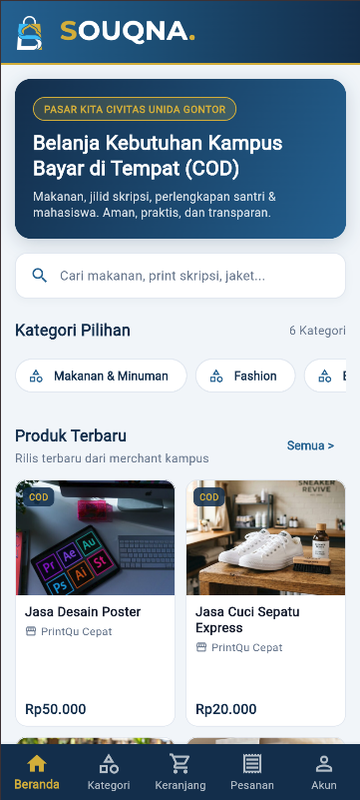
\includegraphics[height=6.7cm]{mockup-beranda.png}
      };
    \end{tikzpicture}\\[0.12cm]
    {\footnotesize\textbf{(A) Beranda Utama}}\\[-0.05cm]
    {\scriptsize\textcolor{unidagray}{Katalog \& banner COD}}
  \end{minipage}
  \hfill
  \begin{minipage}[t]{0.31\textwidth}
    \centering
    \begin{tikzpicture}
      \node[draw=unidaborder, line width=0.8pt, rounded corners=6pt, inner sep=0.5pt, fill=white] {
        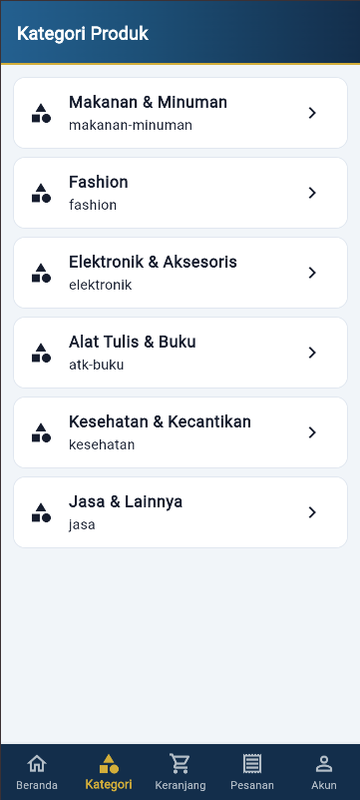
\includegraphics[height=6.7cm]{mockup-kategori.png}
      };
    \end{tikzpicture}\\[0.12cm]
    {\footnotesize\textbf{(B) Kategori Produk}}\\[-0.05cm]
    {\scriptsize\textcolor{unidagray}{6 kategori unit usaha}}
  \end{minipage}
  \hfill
  \begin{minipage}[t]{0.31\textwidth}
    \centering
    \begin{tikzpicture}
      \node[draw=unidaborder, line width=0.8pt, rounded corners=6pt, inner sep=0.5pt, fill=white] {
        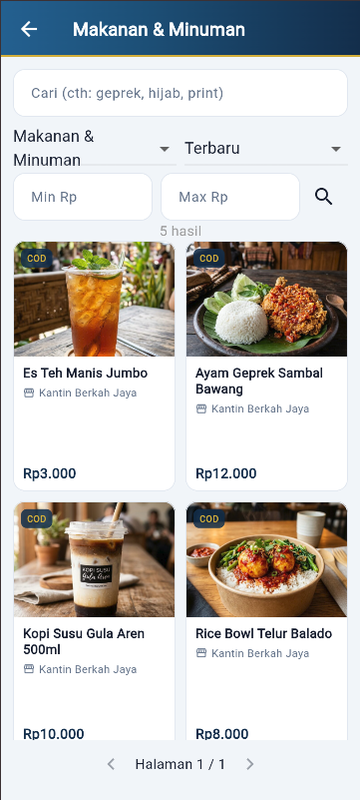
\includegraphics[height=6.7cm]{mockup-produk.png}
      };
    \end{tikzpicture}\\[0.12cm]
    {\footnotesize\textbf{(C) Filter \& Katalog}}\\[-0.05cm]
    {\scriptsize\textcolor{unidagray}{Pencarian \& rentang harga}}
  \end{minipage}

  \vspace{0.35cm}

  % Baris 2: Keranjang, Pesanan Saya
  \begin{minipage}[t]{0.35\textwidth}
    \centering
    \begin{tikzpicture}
      \node[draw=unidaborder, line width=0.8pt, rounded corners=6pt, inner sep=0.5pt, fill=white] {
        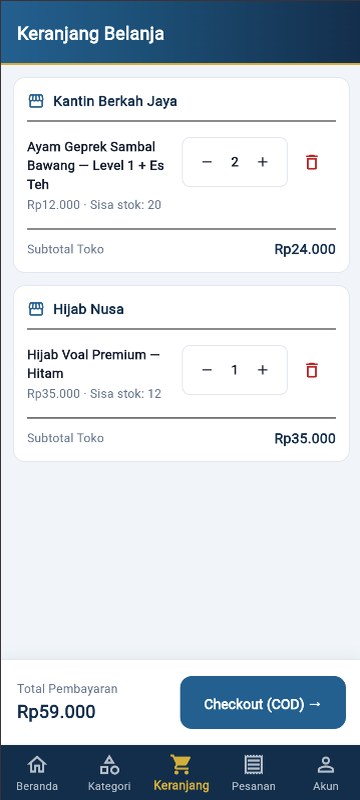
\includegraphics[height=6.7cm]{mockup-keranjang.png}
      };
    \end{tikzpicture}\\[0.12cm]
    {\footnotesize\textbf{(D) Keranjang Belanja}}\\[-0.05cm]
    {\scriptsize\textcolor{unidagray}{Rincian per stan \& checkout COD}}
  \end{minipage}
  \hspace{1.5cm}
  \begin{minipage}[t]{0.35\textwidth}
    \centering
    \begin{tikzpicture}
      \node[draw=unidaborder, line width=0.8pt, rounded corners=6pt, inner sep=0.5pt, fill=white] {
        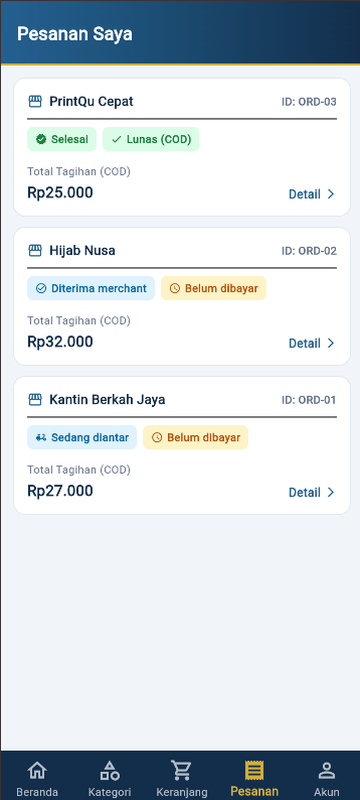
\includegraphics[height=6.7cm]{mockup-pesanan.png}
      };
    \end{tikzpicture}\\[0.12cm]
    {\footnotesize\textbf{(E) Pesanan Saya (COD)}}\\[-0.05cm]
    {\scriptsize\textcolor{unidagray}{Pelacakan status \& bayar di tempat}}
  \end{minipage}
\end{center}

\clearpage

\subsection{Antarmuka Penjual (Merchant / Unit Usaha Kampus)}

\vspace{0.2cm}

\begin{center}
  % Baris 1: Ringkasan Toko & Kelola Produk
  \begin{minipage}[t]{0.42\textwidth}
    \centering
    \begin{tikzpicture}
      \node[draw=unidaborder, line width=0.8pt, rounded corners=6pt, inner sep=0.5pt, fill=white] {
        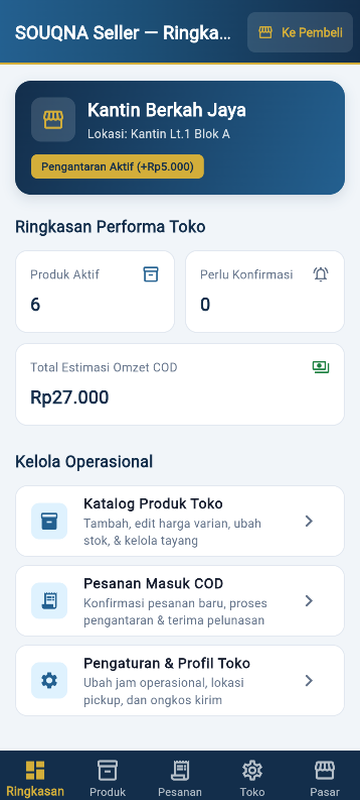
\includegraphics[height=7.2cm]{mockup-seller-ringkasan.png}
      };
    \end{tikzpicture}\\[0.15cm]
    {\footnotesize\textbf{(F) Dasbor \& Performa Toko}}\\[-0.05cm]
    {\scriptsize\textcolor{unidagray}{Ringkasan produk aktif \& omzet COD}}
  \end{minipage}
  \hspace{1.2cm}
  \begin{minipage}[t]{0.42\textwidth}
    \centering
    \begin{tikzpicture}
      \node[draw=unidaborder, line width=0.8pt, rounded corners=6pt, inner sep=0.5pt, fill=white] {
        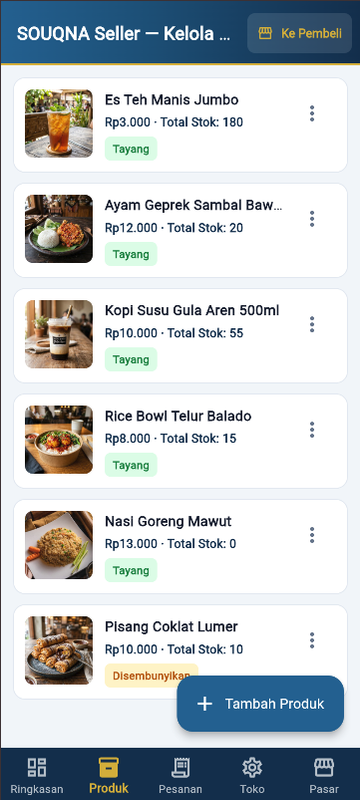
\includegraphics[height=7.2cm]{mockup-seller-produk.png}
      };
    \end{tikzpicture}\\[0.15cm]
    {\footnotesize\textbf{(G) Kelola Produk Toko}}\\[-0.05cm]
    {\scriptsize\textcolor{unidagray}{Daftar etalase, ubah stok \& tambah produk}}
  \end{minipage}

  \vspace{0.45cm}

  % Baris 2: Pesanan Masuk & Pengaturan Toko
  \begin{minipage}[t]{0.42\textwidth}
    \centering
    \begin{tikzpicture}
      \node[draw=unidaborder, line width=0.8pt, rounded corners=6pt, inner sep=0.5pt, fill=white] {
        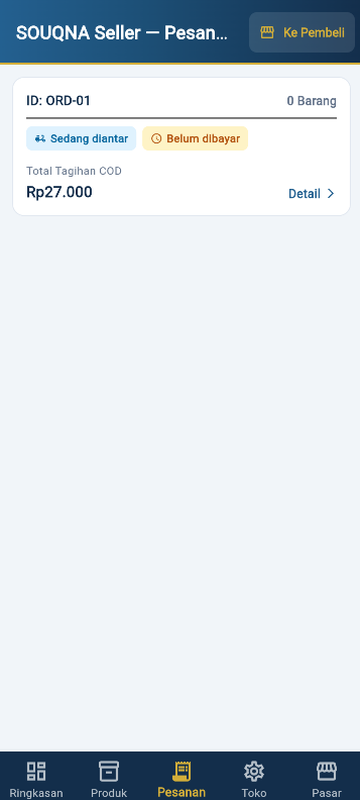
\includegraphics[height=7.2cm]{mockup-seller-pesanan.png}
      };
    \end{tikzpicture}\\[0.15cm]
    {\footnotesize\textbf{(H) Pesanan Masuk COD}}\\[-0.05cm]
    {\scriptsize\textcolor{unidagray}{Konfirmasi pesanan \& status antar}}
  \end{minipage}
  \hspace{1.2cm}
  \begin{minipage}[t]{0.42\textwidth}
    \centering
    \begin{tikzpicture}
      \node[draw=unidaborder, line width=0.8pt, rounded corners=6pt, inner sep=0.5pt, fill=white] {
        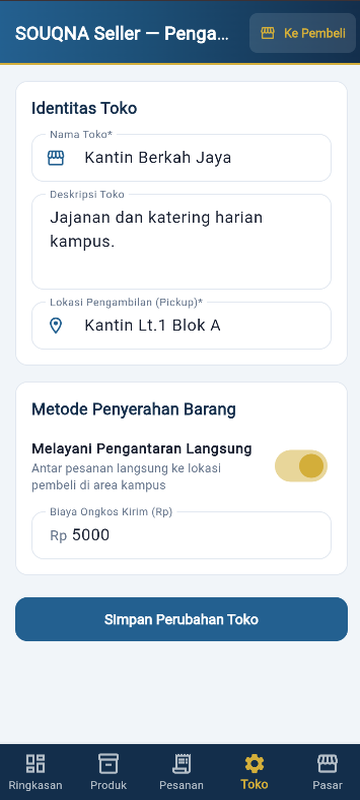
\includegraphics[height=7.2cm]{mockup-seller-toko.png}
      };
    \end{tikzpicture}\\[0.15cm]
    {\footnotesize\textbf{(I) Pengaturan \& Lokasi Toko}}\\[-0.05cm]
    {\scriptsize\textcolor{unidagray}{Titik stan pickup \& ongkir antar kampus}}
  \end{minipage}
\end{center}

\clearpage

%======================================================================================
% 6. RENCANA PENGUJIAN
%======================================================================================
\section{Rencana Pengujian Aplikasi}

Uji dilakukan manual dengan data contoh, cukup 4 skenario yang didemo ke dosen:

\vspace{0.1cm}
\noindent\small
\begin{tabularx}{\textwidth}{@{} c >{\raggedright\arraybackslash}p{3cm} >{\raggedright\arraybackslash}p{4.5cm} >{\raggedright\arraybackslash}X @{}}
\toprule
\textbf{ID} & \textbf{Skenario} & \textbf{Cara Uji} & \textbf{Hasil yang Diharapkan} \\
\midrule
TC-01 & Cari produk &
  Ketik ``geprek'' di pencarian &
  Produk muncul dengan harga dan nama toko yang benar \\
\addlinespace
TC-02 & Beli sampai checkout &
  Masukkan 2 produk 1 toko ke keranjang, tekan Checkout &
  Muncul 1 pesanan dengan total = harga + ongkir \\
\addlinespace
TC-03 & Lacak pesanan &
  Buka detail pesanan, tekan ``Saya Sudah Menerima Barang'' &
  Status berubah menjadi \textit{Selesai} \\
\addlinespace
TC-04 & Kelola unit usaha &
  Buka dasbor toko, ubah stok, simpan &
  Stok baru langsung terlihat di katalog pembeli \\
\bottomrule
\end{tabularx}

\vspace{0.4cm}
\normalsize

\noindent\textbf{Pembagian tugas (2 orang):}
\begin{itemize}
  \item \textbf{Farrel} --- sisi pembeli: beranda, pencarian, detail, keranjang, checkout.
  \item \textbf{Hardi} --- sisi unit usaha + pesanan: dasbor toko, stok, status pesanan, data contoh.
\end{itemize}

\end{document}
